\section{Optimization as the Engine of Learning}

The previous sections described learning in statistical terms: a hypothesis class is chosen, a loss function measures predictive quality, and a learner seeks a model with small empirical risk and, ultimately, small population risk. But this still leaves a practical question unanswered:

\begin{quote}
How is such a model actually found?
\end{quote}

The answer is that, once a model class and objective have been specified, learning usually becomes an optimization problem. Statistical ideas tell us what quantity matters; optimization provides the computational procedure that searches for parameters making that quantity small. In this sense, optimization is the engine that turns a learning principle into an actual algorithm.

\subsection*{From empirical risk to an optimization problem}

Suppose a model is parameterized by $\theta\in\Theta$, so that predictions are made by a function $f_\theta$. Given a dataset
\[
\mathcal D=\{(x_i,y_i)\}_{i=1}^n
\]
and a loss function $\ell$, the empirical risk is
\[
\widehat R_n(f_\theta)=\frac1n\sum_{i=1}^n \ell(f_\theta(x_i),y_i).
\]

\begin{definition}[Optimization problem induced by empirical risk]
The \emph{optimization problem induced by empirical risk} is the problem of finding parameters $\theta$ that minimize a data-dependent objective of the form
\[
J_n(\theta)=\widehat R_n(f_\theta)
\]
or, more generally,
\[
J_n(\theta)=\widehat R_n(f_\theta)+\lambda\,\Omega(\theta),
\]
where $\Omega(\theta)$ is a regularization term and $\lambda\ge 0$ controls its strength.
\end{definition}

Thus, after the modeling choices have been made, the learner faces a numerical search problem:
\[
\min_{\theta\in\Theta} J_n(\theta).
\]
This is the computational side of learning.

\begin{figure}[tbp]
\centering
\begin{tikzpicture}[
    box/.style={draw, rounded corners, fill=gray!10, inner sep=6pt, minimum width=2.8cm, minimum height=1cm},
    arrow/.style={-{Latex[length=2.2mm]}, thick},
    every node/.style={align=center}
]
\node[box] (data) at (0,0) {data\\$\mathcal D$};
\node[box] (loss) at (3.6,0) {loss and model\\$\ell,\ f_\theta$};
\node[box] (obj) at (7.2,0) {objective\\$J_n(\theta)$};
\node[box] (opt) at (10.8,0) {optimizer};
\node[box] (pred) at (14.4,0) {learned predictor\\$f_{\hat\theta}$};

\draw[arrow] (1.45,0) -- (2.15,0);
\draw[arrow] (5.05,0) -- (5.75,0);
\draw[arrow] (8.65,0) -- (9.35,0);
\draw[arrow] (12.25,0) -- (12.95,0);

\node at (7.2,-1.25) {\small learning becomes computationally concrete once empirical risk is turned into an objective to be minimized};
\end{tikzpicture}
\caption{A summary of the optimization viewpoint. Data, model, and loss together define an objective, and optimization produces the learned predictor.}
\end{figure}

\subsection*{Some common objectives}

Different learning tasks lead to different objectives.

\paragraph{Squared loss.}
For regression,
\[
\ell(\hat y,y)=(\hat y-y)^2,
\]
so the empirical objective becomes
\[
J_n(\theta)=\frac1n\sum_{i=1}^n (f_\theta(x_i)-y_i)^2.
\]

\paragraph{Cross-entropy or log loss.}
If the model outputs probabilities $p_\theta(y\mid x)$, then one often uses
\[
\ell(\theta;(x,y))=-\log p_\theta(y\mid x),
\]
which leads to
\[
J_n(\theta)=-\frac1n\sum_{i=1}^n \log p_\theta(y_i\mid x_i).
\]

\paragraph{Regularized objectives.}
To discourage unstable or overly complex solutions, one often minimizes
\[
J_n(\theta)=\widehat R_n(f_\theta)+\lambda\,\Omega(\theta).
\]
For example, $\Omega(\theta)=\|\theta\|_2^2$ gives an $\ell_2$ penalty.

Different losses and penalties create different optimization landscapes. Part of the art of machine learning is choosing objectives that are statistically meaningful and computationally manageable.

\subsection*{Gradient descent}

When the objective is differentiable, the basic local method is gradient descent.

\begin{definition}[Gradient descent]
Let $J:\Theta\to\mathbb R$ be differentiable. Starting from an initial point $\theta_0$, \emph{gradient descent} generates iterates
\[
\theta_{t+1}=\theta_t-\eta_t \nabla J(\theta_t),
\]
where $\eta_t>0$ is the learning rate or step size.
\end{definition}

The geometric intuition is that $\nabla J(\theta_t)$ points in the direction of steepest local increase of the objective, so its negative points toward steepest local decrease.

\begin{proposition}[Negative gradient is the direction of steepest local decrease]
Let $J:\mathbb R^d\to\mathbb R$ be differentiable at $\theta$, and let $u$ be any unit vector. Then the directional derivative of $J$ at $\theta$ in direction $u$ is
\[
D_u J(\theta)=\nabla J(\theta)^\top u.
\]
Among all unit directions $u$, this quantity is minimized when
\[
u=-\frac{\nabla J(\theta)}{\|\nabla J(\theta)\|}
\]
provided $\nabla J(\theta)\neq 0$. The minimum value is
\[
-\|\nabla J(\theta)\|.
\]
\end{proposition}

\begin{proof}
For a unit vector $u$, the directional derivative is
\[
D_u J(\theta)=\nabla J(\theta)^\top u.
\]
By the Cauchy--Schwarz inequality,
\[
\nabla J(\theta)^\top u \ge -\|\nabla J(\theta)\|\,\|u\|=-\|\nabla J(\theta)\|.
\]
Equality holds when $u$ points exactly opposite to the gradient, that is,
\[
u=-\frac{\nabla J(\theta)}{\|\nabla J(\theta)\|}.
\]
Hence the negative gradient gives the direction of steepest local decrease.
\end{proof}

This proposition explains why gradients are so useful in high dimensions. Instead of searching blindly over many possible directions, the gradient gives a principled local direction of improvement.

\subsection*{A worked one-dimensional example}

Consider the one-dimensional objective
\[
J(\theta)=\frac12(\theta-3)^2.
\]
Then
\[
J'(\theta)=\theta-3.
\]
Gradient descent with a fixed learning rate $\eta$ gives
\[
\theta_{t+1}=\theta_t-\eta(\theta_t-3).
\]

If we choose $\eta=\frac12$ and start from $\theta_0=0$, then
\[
\theta_1=0-\frac12(0-3)=\frac32,
\]
\[
\theta_2=\frac32-\frac12\left(\frac32-3\right)=\frac94,
\]
\[
\theta_3=\frac94-\frac12\left(\frac94-3\right)=\frac{21}{8}.
\]
The iterates move toward $\theta=3$, which is the minimizer.

This example is simple, but it already shows the key idea: optimization proceeds by repeated local corrections based on derivative information.

\begin{figure}[tbp]
\centering
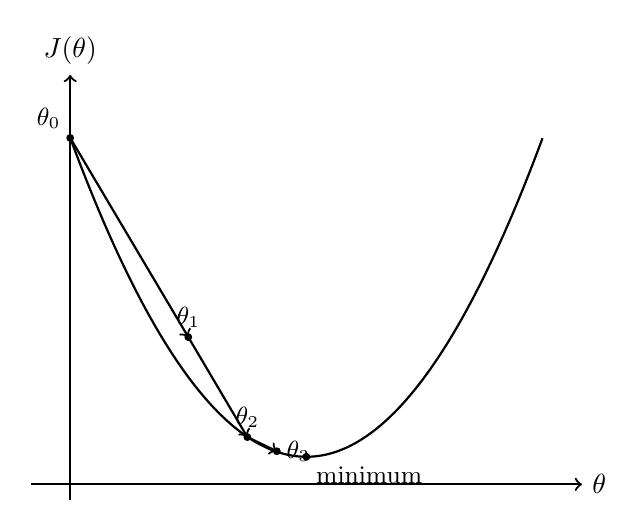
\begin{tikzpicture}[scale=1, every node/.style={align=center}]
    \draw[->, thick] (-0.5,0) -- (6.5,0) node[right] {$\theta$};
    \draw[->, thick] (0,-0.2) -- (0,5.2) node[above] {$J(\theta)$};

    \draw[thick, domain=0:6, samples=100] plot (\x,{0.45*(\x-3)^2+0.35});

    \filldraw (0,4.4) circle (1.2pt) node[above left] {\small $\theta_0$};
    \filldraw (1.5,1.87) circle (1.2pt) node[above] {\small $\theta_1$};
    \filldraw (2.25,0.60) circle (1.2pt) node[above] {\small $\theta_2$};
    \filldraw (2.625,0.42) circle (1.2pt) node[right] {\small $\theta_3$};
    \filldraw (3,0.35) circle (1.2pt) node[below right] {\small minimum};

    \draw[->, thick] (0,4.4) -- (1.5,1.87);
    \draw[->, thick] (1.5,1.87) -- (2.25,0.60);
    \draw[->, thick] (2.25,0.60) -- (2.625,0.42);
\end{tikzpicture}
\caption{A one-dimensional loss landscape. Gradient descent updates move iteratively downhill toward a minimizer.}
\end{figure}

\subsection*{Stochastic gradient descent}

For large datasets, computing the full gradient of
\[
J_n(\theta)=\frac1n\sum_{i=1}^n \ell(f_\theta(x_i),y_i)
\]
may be expensive. Indeed,
\[
\nabla J_n(\theta)=\frac1n\sum_{i=1}^n \nabla_\theta \ell(f_\theta(x_i),y_i),
\]
which requires a pass through the entire training set at every step.

A cheaper alternative is to approximate the gradient using only a small part of the sample.

\begin{definition}[Stochastic gradient descent]
\emph{Stochastic gradient descent} (SGD) updates the parameters using a random gradient estimate:
\[
\theta_{t+1}=\theta_t-\eta_t g_t,
\]
where $g_t$ is computed from a randomly chosen example or minibatch. For a single sampled example $(x_i,y_i)$, one may take
\[
g_t=\nabla_\theta \ell(f_{\theta_t}(x_i),y_i).
\]
\end{definition}

If the example is sampled uniformly at random, then
\[
\mathbb E[g_t\mid \theta_t]=\nabla J_n(\theta_t),
\]
so the stochastic update is noisy but unbiased with respect to the empirical objective.

\begin{figure}[tbp]
\centering
\begin{tikzpicture}[
    box/.style={draw, rounded corners, fill=gray!10, inner sep=6pt, minimum width=3.2cm, minimum height=1cm},
    arrow/.style={-{Latex[length=2.2mm]}, thick},
    every node/.style={align=center}
]
\node[box] (full) at (0,0) {full-batch gradient descent\\uses all $n$ examples};
\node[box] (sgd) at (5.5,0) {SGD\\uses one random example};
\node[box] (mini) at (11,0) {minibatch SGD\\uses a small random batch};

\draw[arrow] (1.6,-0.75) -- (1.6,-2.2);
\draw[arrow] (7.1,-0.75) -- (7.1,-2.2);
\draw[arrow] (12.6,-0.75) -- (12.6,-2.2);

\node at (1.6,-2.8) {\small accurate gradient\\high cost per step};
\node at (7.1,-2.8) {\small very cheap\\high noise};
\node at (12.6,-2.8) {\small practical compromise\\moderate noise};

\end{tikzpicture}
\caption{Full-batch gradient descent, single-example SGD, and minibatch SGD. Modern training usually uses minibatches because they balance computational cost and gradient quality.}
\end{figure}

\subsection*{Minibatches and gradient noise}

In practice, one usually uses a minibatch $B_t\subset\{1,\dots,n\}$ and forms
\[
g_t=\frac1{|B_t|}\sum_{i\in B_t}\nabla_\theta \ell(f_{\theta_t}(x_i),y_i).
\]
This gives a compromise between two extremes:

\begin{itemize}
    \item full-batch gradients are accurate but expensive;
    \item single-example gradients are cheap but noisy.
\end{itemize}

The noise is not merely a nuisance. It is part of the dynamics of modern optimization. The estimated gradient fluctuates from step to step because different minibatches contain different examples.

\begin{figure}[tbp]
\centering
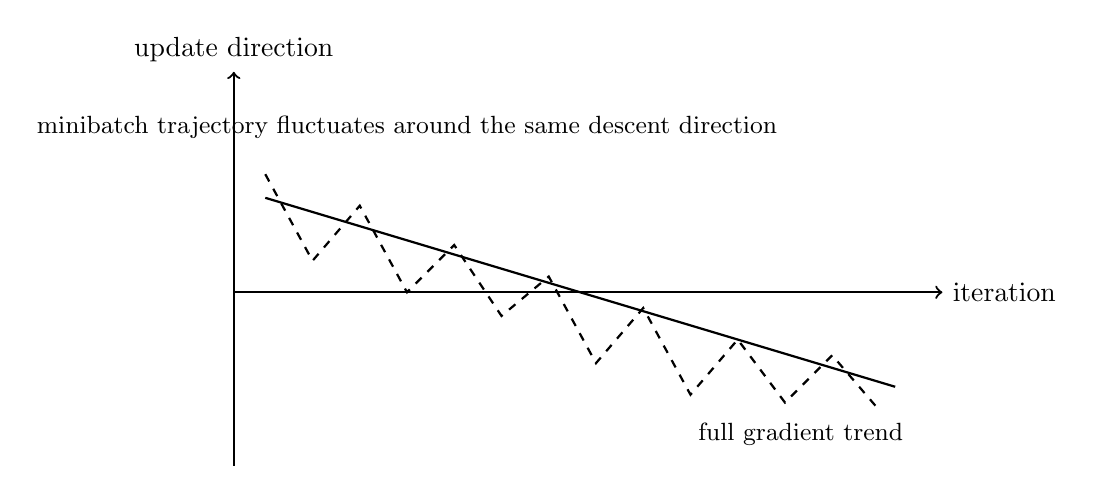
\begin{tikzpicture}[scale=1, every node/.style={align=center}]
    \draw[->, thick] (0,0) -- (9,0) node[right] {iteration};
    \draw[->, thick] (0,-2.2) -- (0,2.8) node[above] {update direction};

    \draw[thick] (0.4,1.2) -- (8.4,-1.2);
    \node at (7.2,-1.8) {\small full gradient trend};

    \draw[thick, dashed]
        (0.4,1.5) -- (1.0,0.4) -- (1.6,1.1) -- (2.2,0.0) -- (2.8,0.6) --
        (3.4,-0.3) -- (4.0,0.2) -- (4.6,-0.9) -- (5.2,-0.2) -- (5.8,-1.3) --
        (6.4,-0.6) -- (7.0,-1.4) -- (7.6,-0.8) -- (8.2,-1.5);
    \node at (2.2,2.1) {\small minibatch trajectory fluctuates around the same descent direction};
\end{tikzpicture}
\caption{Minibatch noise intuition. A stochastic gradient follows the overall downhill trend only approximately, with fluctuations caused by sampling different subsets of data.}
\end{figure}

\subsection*{Learning rates and the scale of updates}

The learning rate $\eta_t$ determines how far the algorithm moves in the chosen direction. If it is too small, progress may be extremely slow. If it is too large, the algorithm may overshoot, oscillate, or diverge.

Thus optimization is not only about the direction of motion but also about its scale. Later chapters will revisit this when we discuss signal propagation, initialization, and optimization in deep networks.

\subsection*{A convexity intuition}

Some classical learning objectives are convex, and convexity gives a particularly clean optimization picture.

\begin{proposition}[Local minima are global for convex functions]
Let $J:\Theta\to\mathbb R$ be convex on a convex set $\Theta$. Then every local minimizer of $J$ is also a global minimizer.
\end{proposition}

\begin{proof}
Suppose $\theta^\star$ is a local minimizer but not a global minimizer. Then there exists $\theta\in\Theta$ such that
\[
J(\theta)<J(\theta^\star).
\]
For $0<\lambda<1$, convexity gives
\[
J\big((1-\lambda)\theta^\star+\lambda\theta\big)
\le
(1-\lambda)J(\theta^\star)+\lambda J(\theta)
<
J(\theta^\star).
\]
For sufficiently small $\lambda$, the point $(1-\lambda)\theta^\star+\lambda\theta$ lies arbitrarily close to $\theta^\star$, contradicting the assumption that $\theta^\star$ is a local minimizer. Therefore every local minimizer must be global.
\end{proof}

This helps explain why convex models such as linear regression and logistic regression are mathematically attractive. Their optimization landscapes are simpler to reason about than the highly nonconvex landscapes of deep networks.

\subsection*{Optimization is not generalization}

A central lesson of machine learning is that optimization and generalization are related but distinct.

\paragraph{Optimization question.}
Can we find parameters that make the training objective small?

\paragraph{Generalization question.}
Will those parameters perform well on new data?

These are not the same question. A model can be optimized successfully and still generalize poorly if it overfits the training sample. Conversely, a model may be difficult to optimize but still have good predictive potential if a good solution can be found.

\commonconfusion{Low training loss is not identical to good generalization. Optimization concerns how well we reduce the chosen objective on the training data. Generalization concerns whether the resulting predictor performs well on fresh data. Confusing the two leads to one of the most common misunderstandings in machine learning.}

\whattoremember{Once a model and loss have been chosen, learning usually becomes an optimization problem. Gradient descent follows the negative gradient because it is the direction of steepest local decrease. Stochastic gradient descent replaces the full gradient by a cheaper random estimate, and minibatches provide the practical compromise used in modern training. Optimization determines how low the training objective becomes, but low training loss by itself does not guarantee good prediction on new data.}

\subsection*{Exercises}

\begin{exercise}
Let
\[
J(\theta)=\frac12(\theta-5)^2.
\]
Compute $J'(\theta)$ and write the gradient descent update with learning rate $\eta$. Starting from $\theta_0=1$, compute $\theta_1$ and $\theta_2$ when $\eta=\frac12$.
\end{exercise}

\begin{exercise}
Consider the linear model
\[
f_\theta(x)=\theta x
\]
with squared loss on a single example $(x,y)$. Show that
\[
\ell(\theta;(x,y))=(\theta x-y)^2
\]
has derivative
\[
\frac{d}{d\theta}\ell(\theta;(x,y))=2x(\theta x-y).
\]
\end{exercise}

\begin{exercise}
Explain in words why the negative gradient is a sensible update direction for a differentiable objective.
\end{exercise}

\begin{exercise}
What is the practical difference between full-batch gradient descent and stochastic gradient descent? What is the role of a minibatch?
\end{exercise}

\begin{exercise}
Give an example of a situation in which a model achieves very low training loss but still generalizes poorly. Which concept from the previous section does this illustrate?
\end{exercise}

\begin{exercise}
Why does convexity make optimization easier to reason about, at least conceptually, than a general nonconvex objective?
\end{exercise}

\subsection*{Notes and references}

This section introduces the optimization viewpoint that turns empirical risk minimization into an algorithmic problem. The role of gradient descent, SGD, minibatches, learning rates, and convexity will recur throughout the book. At this stage the emphasis is conceptual: optimization is the computational mechanism by which learning occurs, but it does not by itself explain why learned models generalize. Chapter 2 will revisit these ideas in the richer setting of neural networks, backpropagation, signal propagation, and the training of deep models.